\chapter{Methodology}

\section{Hasing module}

\subsection{Test Setup}
In order to evaluate the performance increase obtained when using a dedicated
hashing accelerator, a test system was constructed using Xilinx' Vivado
development studio.

\begin{figure}[ht]
	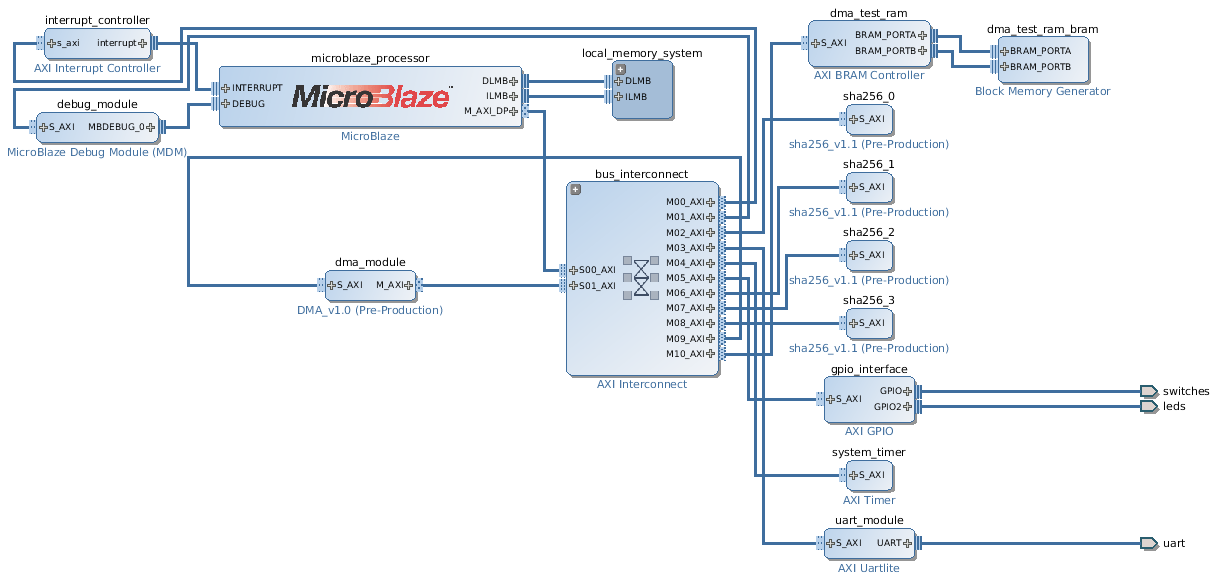
\includegraphics[width=0.95\textwidth]{Figures/testsystem-vivado.png}
	\caption{Overview of the test system}
	\label{fig:testsystem-vivado}
\end{figure}

The test system is controlled by a MicroBlaze microprocessor, configured to
include the optional barrel shifter, integer divider and pattern comparator.
In order to run the XilKernel real-time operating system, the system also
includes a simple timer module for use by the kernel.

A UartLite module was included to provide I/O in order to communicate with
the system from a desktop computer, as well as a GPIO module for additional
debugging use.

The system runs on a 50~MHz clock which is synthesized by a clock generator
module from a 100~MHz input clock.

In order to run performance tests on the system, the DMA described in
section \ref{undefined}\todo{Insert correct reference here} and four
SHA256 hashing modules are included.\todo{Maybe reduce to one now}
A fixed-interval timer, that generates an interrupt every second, is
included in order to calculate the performance per second.

\subsection{Test Software}
In order to test the hashing modules and how the performance scales when including
multiple hashing modules, a benchmark application was written. The benchmark
runs a specified number of threads that tries to hash a single block of data
over and over again.

A simple scheduler is used to provide each thread with an available hashing module.
If no module is available, the thread blocks on a semaphore until a module is available.

Once a second, the number of completed hashes for each module is added up and
reported over the UART.

The test software is also designed so that it can be run with a software implementation
of the hashing algorithm instead of the hashing modules. This makes it possible
to compare the performance when using an accelerator as compared to not using
an accelerator.

\subsection{Measurements and Benchmarks}
The most important performance measure for a Bitcoin mining system is the number
of hashes per second it can sustain. Therefore, once a second the number of hashes
computed since the previous second is calculated and sent over the UART.

Another important measurement is how the inclusion of a DMA affects the performance
of the system.

\subsection{Theoretical Maximum Performance} % This section can be moved elsewhere

The hashing modules can finish one round of hashing in 65 clock cycles. If
every hash can be obtained from only one block of data, it is possible to
obtain a hash every 65 clock cycles under ideal conditions. This translates
into a maximum theoretical performance of 768230~H/s at a clock frequency of
50~MHz.

However, the modules do not exist in a vacuum, and data needs to be transferred
between the modules and a controller, such as a microprocessor. The hashing tiles
are connected to the rest of the system using an AXI4 lite interface. Transfers
on the AXI bus takes at least three cycles for writes and two cycles for reads,
if it is assumed that no burst transfers are used\footnote{Indeed, the AXI4 lite
interface only allows burst lengths of one word, in essence no burst transfer is
supported.}

In order for the hashing module to word, it needs 16 32-bit words of input data,
and control signals must be set up. This causes at least 17 words of data to
need to be written to the module, taking at least 51 clock cycles. Then, after
hashing of a block is complete, if there are no more blocks, the result must
be read back. The result consists of 8 words of data, which takes at least 16
clock cycles to transfer.

In total, a minimum of 67 clock cycles of overhead is needed per hash when assuming
a one-block input size and an ideal AXI4 bus. Not considering the additional overhead
from processing in the microprocessor, such as when handlig the interrupt when the
hashing finishes, hashing may take a minimum of $67 + 65 = 132$ clock cycles to
complete, bringing the maximum theoretical performance down to at most 378787~H/s.

However, in a real system, there are many additional sources of overhead reducing
the performance additionally.\todo{Maybe move this somewhere else}

\section{Testing and verification of DMA Module}
The DMA Module is tested by first testing individual components, then their interaction with each other.

In the individual testing, the component receives different combinations of the inputs as the time passes.
The test shows whether the component behaves as expected, based on the input.
This is done by reading the outputs based on inputs and/or values of internal registers.
Components that are tested individually are:
\begin{itemize}
    \item \textbf{Adapter} 
    \item \textbf{Arbiter Controller}
    \item \textbf{DMA Main Controller}
    \item \todo{Eeehh...} FIFO buffers are tested during design of HASH-module. 
    \item \textbf{Load Channel}
    \item \textbf{Store Channel}
\end{itemize}

In the interaction testing, also known as topview-testing, the components are tested for their interaction with each other.
Since the components have been tested individually, they are assumed at this point to be functional. 
Internal values are thus ignored, also since the focus of the tests are to ensure that the interaction between the components are working as expected.
The interaction tests are:
\begin{itemize}
    \item \textbf{Arbiter} - Tests that internal multiplexers are set correctly by the controller, based on the selected requests.
    \item \textbf{Two Channel setup, signle request} - First of two tests that checks if the two-channel setup works as expected, by activating a single channel.
    Data with ID is fed manually to the data buffer.
    The tests ensures that a load channel sends out number of requests according to count value, and that whenever data arrives, stores are issued and get priority above loads.
    Also tests if interrupts and blocks get highest priority, and that active signals are activated and deactivated correctly.
    \todo{This is actually just saying that I didn't add separate counters here as I did in the topview test for the entire module}
    Correctness is ensured by reading the output values (mainly detailsoutput and dataOutput) from the two-channel setup.
    \item \textbf{Two Channel setup, two requests} - Second of two tests, this one activates both channels.
    In addition to the first test, this one also ensures that loads from both channels alternates when both are active, and that correct channel identifies and stores the correct data that has been loaded.
    When one channel is done, the other channel will have full access to the arbiter, and loads will no longer alternate.
    Correctness is ensured by reading the output values. 
    \item \textbf{Two Channel setup, two requests} - Second of two tests, this one activates both channels.
    In addition to the first test, this one also ensures that loads from both channels alternates when both are active, and that correct channel identifies and stores the correct data that has been loaded.
    When one channel is done, the other channel will have full access to the arbiter, and loads will no longer alternate.
    Correctness is ensured by reading the output values.
    \item \textbf{Topview} - This is where the entire DMA Module is tested, as requests are sent in.
    Each cycle with load, store, interrupt and blocking are counted (either identified by the command value, or by the blocking signal when it is high, in the test).
    For each load issued, a register receives the load address, and sends it back to the DMA Module with a push signal and data (since the data value is not important for this test, each value is incremented by 8).
    Thus there is a cycle delay from a load is issued to the data arrives to the DMA Module.
    In the real world, there will be far more cycles from a load is issued, until it's data arrives in the DMA Module.
    And issuing multiple loads or not also depends on the system it is integrated with.
    There will be great difference between this project, where the DMA Module is connected to a single shared bus network, and to integrate it on SHMAC, where the main network is switched-media network.
    In this test, however, all data arrives quickly, as if using a bus and memory that is extremely fast.
    One reason is to cut down the necessary waiting time in the test itself, and another is that the module is tested for near-maximum peak.
    There are three tests in total: One with single request (only one channel active), one with two requests (both channels active) and one with four requests (test for waiting requests).
    Correctness is ensured by comparing the test counter values with expected number of loads, stores, interrupts issued, and number of blocks.
    
    \todo{HHHHHHMMMMMMM!!!!!}A word of warning: It turns out in the tests that for each round of blocks, the block counter counts one block less than the number of cycles a block is active. It still turns out, when analysing the signals, that the module is inactive in correct number of cycles as long as the block signal is active, the block counter merely does not count for the first cycle during a block. Since this is considered a flaw with the test itself, and not with the DMA Module, the error is considered negligable. 
\end{itemize}

\todo{Write about testing with the c-coding (ordering a data transfer), and running on FPGA}
KRISTIAN HERE
